\documentclass[10pt,t]{beamer}

\usepackage[utf8]{inputenc}
\usepackage[T1]{fontenc}
\usepackage{graphicx}
\usepackage[caption=false]{subfig}
\usepackage{grffile}
\usepackage{longtable}
\usepackage{wrapfig}
\usepackage{rotating}
\usepackage[normalem]{ulem}
\usepackage{amsmath}
\usepackage{textcomp}
\usepackage{amssymb}
\usepackage{capt-of}
\usepackage{hyperref}

%\newcommand{\nitrous}{N$_2$O\xspace}
%\newcommand{\ozone}{O$_3$\xspace}

\input beamer_setup

\usetheme{default}
% ---------------------------------------------------------------------
% ---------------------------------------------------------------------
\begin{document}

\title[]{AIRS/CrIS Radiance Inter-Calibration: \newline
  Tests of Trends Using Time Series Combining Both Sensors}
\author{Chris Hepplewhite, Howard Motteler, Larrabee Strow}
\institute{Department of Physics, JCET\\
  University of Maryland Baltimore County (UMBC)}
\date{October 2, 2018}
% ---------------------------------------------------------------------
% ---------------------------------------------------------------------
\begin{frame}
  \titlepage
\end{frame}
% ---------------------------------------------------------------------
\begin{frame}
  \frametitle{Overview}
  \begin{itemize}
  \item A Hyperspectral IR climate record depends on sensor continuity
  \item Spectral : AIRS, CrIS, IASI SRFs/ILS Very Different
  \item Radiometric : Differences in the 0.3K or less range, great starting point.
  \item Spatial : AIRS footprint slightly smeared relative to CrIS, slight impact on extrema.
    \item Sampling : AIRS/CrIS sample the globe at slightly different times and atmospheric paths.  Strategies to mitigate exist.
    \item We examine radiometric differences between AIRS and SNPP/NOAA20 CrIS, using both SNOs and statstical sampling.

  \end{itemize}
\end{frame}
% ------------------------------------------------------------------------------
\begin{frame}
  \frametitle{Spectral Considerations}

  \begin{itemize}
  \item Convert AIRS to the CrIS ILS/SRF.  Presently using NSR, will switch in future to something close to 0.8/0.6/0.4 OPD ``CrIS Hybrid'', or ``CHIRP''
  \item Need AIRS L1c (at the DAAC) for production of AIRS2CrIS products.
    % \item Works well because AIRS SRFs are quite uniformly spaced, gaps filled and spectral overlap in wings of SRFs.
  % \item Present approach: standardize on CrIS normal spectral resolution (NSR) for radiometric climate record.
  \item Conversion of IASI2CrIS is essentially trivial since IASI L1c gaussian apodization is far from zero at 0.8 cm path difference, so conversion to 0.8 sinc ILS is robust.
    \end{itemize}

\end{frame}
% -----------------------------------------------------------------------------
\begin{frame}
  \frametitle{Radiometric Considerations}
  \begin{itemize}
    \item AIRS CrIS SNO's global, but heavily weighted to high latitudes
    \item At minimum, we want best statistical match between sensors.  We use equal-area weighted set (1\% of 2016 scenes) sampled over all scan angles.
    \item All scan angle required to keep AIRS and CrIS mean sampling times as close as possible.
    \item AIRS and CrIS have slightly different mean scan (secant) angles.  Easy to correct AIRS to CrIS mean secant, magnitude $\sim$0.2K
  \item We get very good agreement between SNOs and statistical comparisons, giving us some confidence that the instrument differences are not too scene dependent.
  \end{itemize}
  
\end{frame}
% ----------------------------------------------------------------------------

\begin{frame}
  \frametitle{Example of One Month of AIRS:CrIS SNOs: Maps}
  \begin{center}
    \includegraphics[width=0.95\linewidth]{./Figs/sno_ac1_lr_900wvn_aug2018_maps.pdf}
  \end{center}
  
\end{frame}
% --------------------------------------------------------------------
\begin{frame}
  \frametitle{Example of One Month of AIRS:CrIS SNOs: Bias}
  \begin{center}
    \includegraphics[width=0.95\linewidth]{./Figs/sno_ac1_lr_lw_mean_bias_jul2018.pdf}
  \end{center}
  
\end{frame}
% --------------------------------------------------------------------
\begin{frame}
  \frametitle{NPP vs N20 CrIS Using AIRS for Transfer}
  \begin{center}
    \includegraphics[width=0.7\linewidth]{./Figs/sno_march2018_snpp_minus_noaa20_with_c2_airs_ingrey.pdf}
  \end{center}
\begin{small}
  \begin{itemize}
  \item AIRS is used as a cross-calibration transfer standard since no SNOs between SNPP and NOAA20
  \item CrIS and AIRS calibrations still being worked by respective teams
  \end{itemize}
\end{small}  
\end{frame}
% --------------------------------------------------------------------
\begin{frame}
  \frametitle{NPP.CrIS and N20.CrIS Differences by FOV (via AIRS)}
  \begin{center}
\includegraphics[width=0.85\linewidth]{./Figs/sno_ac1_ac2_dble_diff_lr_mw_cfov_2018febjun.pdf}
  \end{center}
\small Bad AIRS channels past 1500 wavenumbers not masked out...  
\end{frame}
% --------------------------------------------------------------------
\begin{frame}
  \frametitle{NPP.CrIS and N20.CrIS Differences by FOV (via IASI)}
  \begin{center}
    \includegraphics[width=0.85\linewidth]{./Figs/sno_i1c1_i1c2_dble_diff_lr_mw_2018febjun_aslp.pdf}
  \end{center}
\small Very similar to differences using AIRS (previous slide)  
\end{frame}
% % --------------------------------------------------------------------
% \begin{frame}
%   \frametitle{How about MetOp-A/B IASI and NPP/N20 CrIS SNOs}
%   \begin{center}
%     \includegraphics[width=0.95\linewidth]{./Figs/sno_iasi_cris_all_combin_mean_bias_spectral.png}
%   \end{center}
  
% \end{frame}
% --------------------------------------------------------------------
% \begin{frame}
%   \frametitle{AIRS:NPP.CrIS SNO and Random Stats Biases}
%   \begin{figure}
%     \centering
%     \subfloat[2016 SNOs]{{\includegraphics[width=5cm]{./Figs/snpp_vs_airs_sno.pdf} }}
%     \qquad
%     \subfloat[2016 Stats]{{\includegraphics[width=5cm]{./Figs/snpp_vs_airs_stats.pdf} }}
%   \end{figure}

%   \small
%   SNOs and random comparisons are in good agreement. Random averages are corrected to compensate for the larger mean secant viewing angle of CrIS vs AIRS and compared to SNOs.
% \end{frame}
% --------------------------------------------------------------------
% ---------------------------------------------------------------------
\begin{frame}
\frametitle{AIRS:NPP.CrIS SNO and Random Stats Biases}
\vspace{-0.2in}
\begin{columns}
  \begin{column}{0.55\columnwidth}
      \begin{block}{2016 SNOs}
\vspace{-0.15in}
        \begin{center}
          \includegraphics[width=\linewidth]{./Figs/snpp_vs_airs_sno.pdf}
        \end{center}
      \end{block}
    \end{column}

    \begin{column}{0.55\columnwidth}
      \begin{block}{2016 Stats}
\vspace{-0.15in}
        \begin{center}
          \includegraphics[width=\linewidth]{./Figs/snpp_vs_airs_stats.pdf} 
        \end{center}
      \end{block}
    \end{column}
  \end{columns}
  \small
  \begin{itemize}
  \item SNOs and random comparisons are in good agreement.
  \item Statistical comprisons are corrected larger mean secant viewing angle of CrIS
  \end{itemize}
\end{frame}
% % --------------------------------------------------------------------
% \begin{frame}
%   \frametitle{AIRS:NPP.CrIS SNO and Random Stats Biases}
%   \begin{figure}
%     \centering
%     \subfloat[2016 SNOs]{{\includegraphics[width=5cm]{./Figs/snpp_vs_airs_sno.pdf} }}
%     \qquad
%     \subfloat[2016 Stats]{{\includegraphics[width=5cm]{./Figs/snpp_vs_airs_stats.pdf} }}
%   \end{figure}

%   \small
%   SNOs and random comparisons are in good agreement. Random averages are corrected to compensate for the larger mean secant viewing angle of CrIS vs AIRS and compared to SNOs.
% \end{frame}
% --------------------------------------------------------------------
\begin{frame}
  \frametitle{Multi-year Mission Overlap Permits Bias Trending}
  \vspace{-0.15in}
  \begin{block}{\footnotesize CrIS vs AIRS}
    \begin{center}
  \vspace{-0.15in}      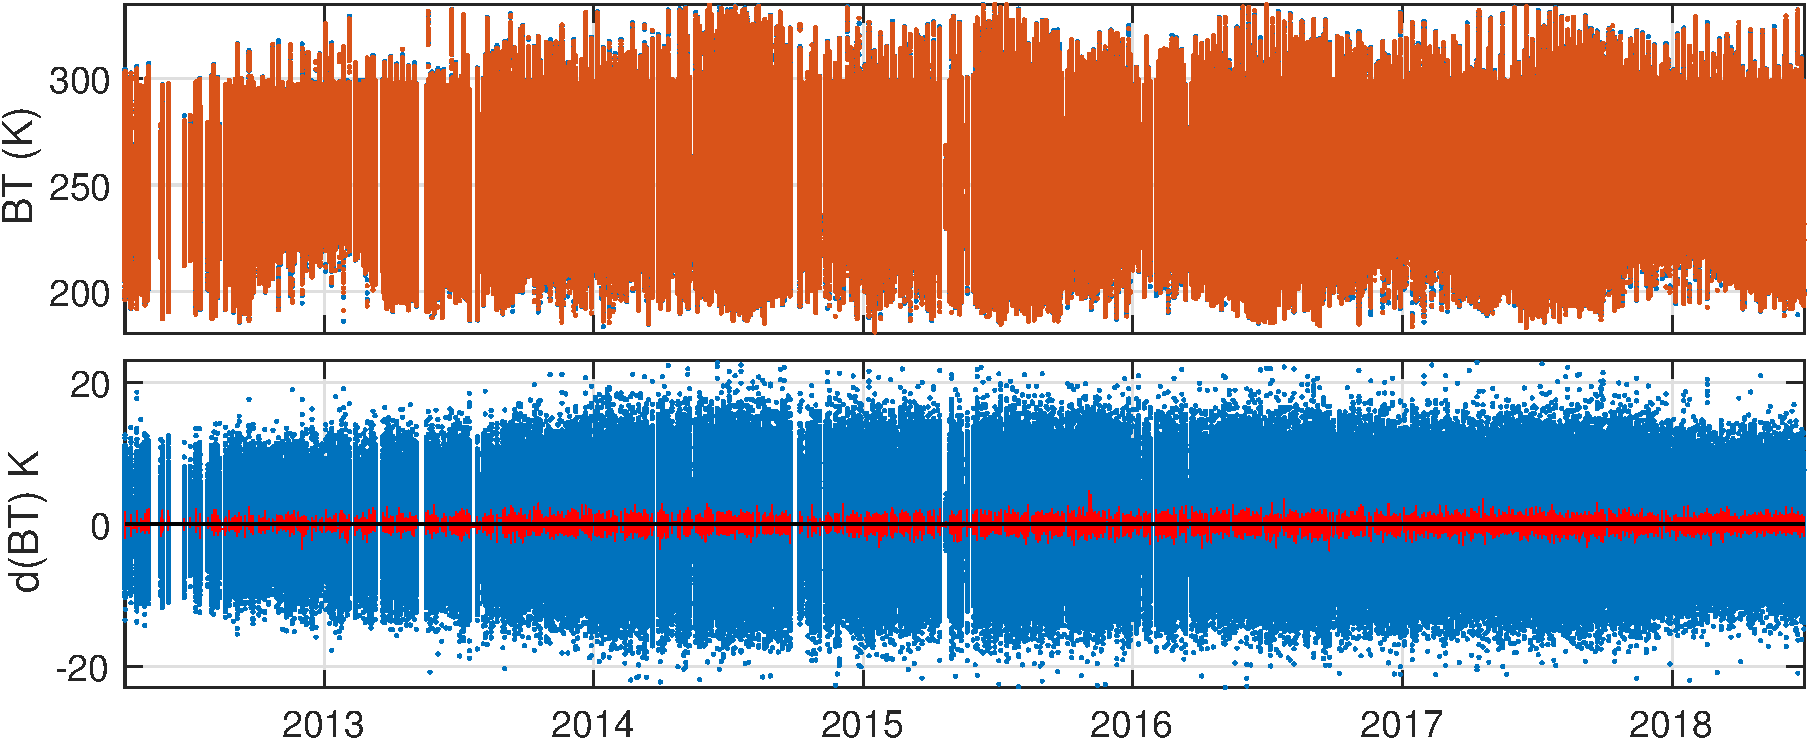
\includegraphics[width=0.7\linewidth]{./Figs/sno_ac1_lr_lw_window_trend_2012_18.png}
    \end{center}
  \end{block}
  \vspace{-0.2in}
  \begin{block}{\footnotesize CrIS vs IASI}
  \vspace{-0.15in}
    \begin{center}
      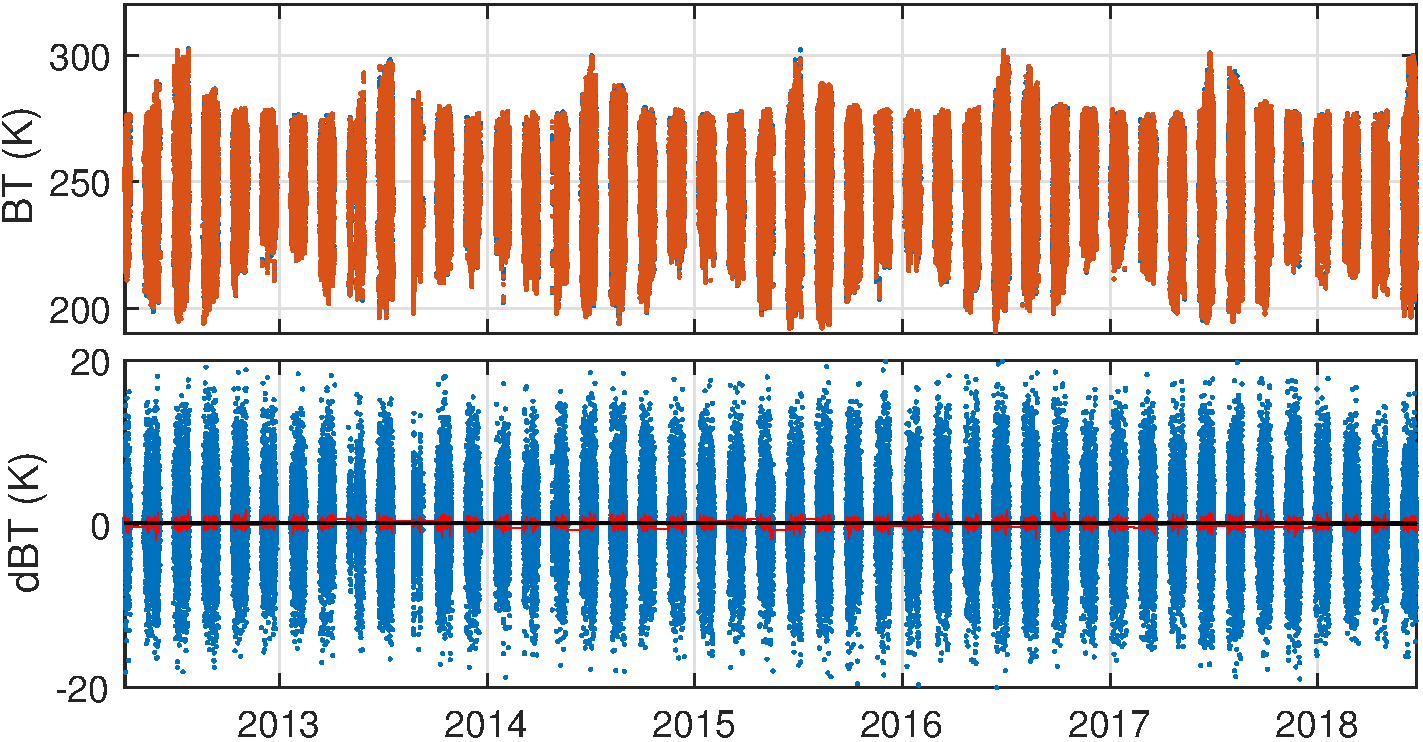
\includegraphics[width=0.7\linewidth]{./Figs/sno_i1c1_lr_lw_window_trend.png}
    \end{center}
  \end{block}
\end{frame}
% % --------------------------------------------------------------------
% \begin{frame}
%   \frametitle{Multi-year Mission Overlap Permits Bias Trending}
%   \begin{figure}[]
%     \subfloat[AIRS:CrIS 900wvn]{
%       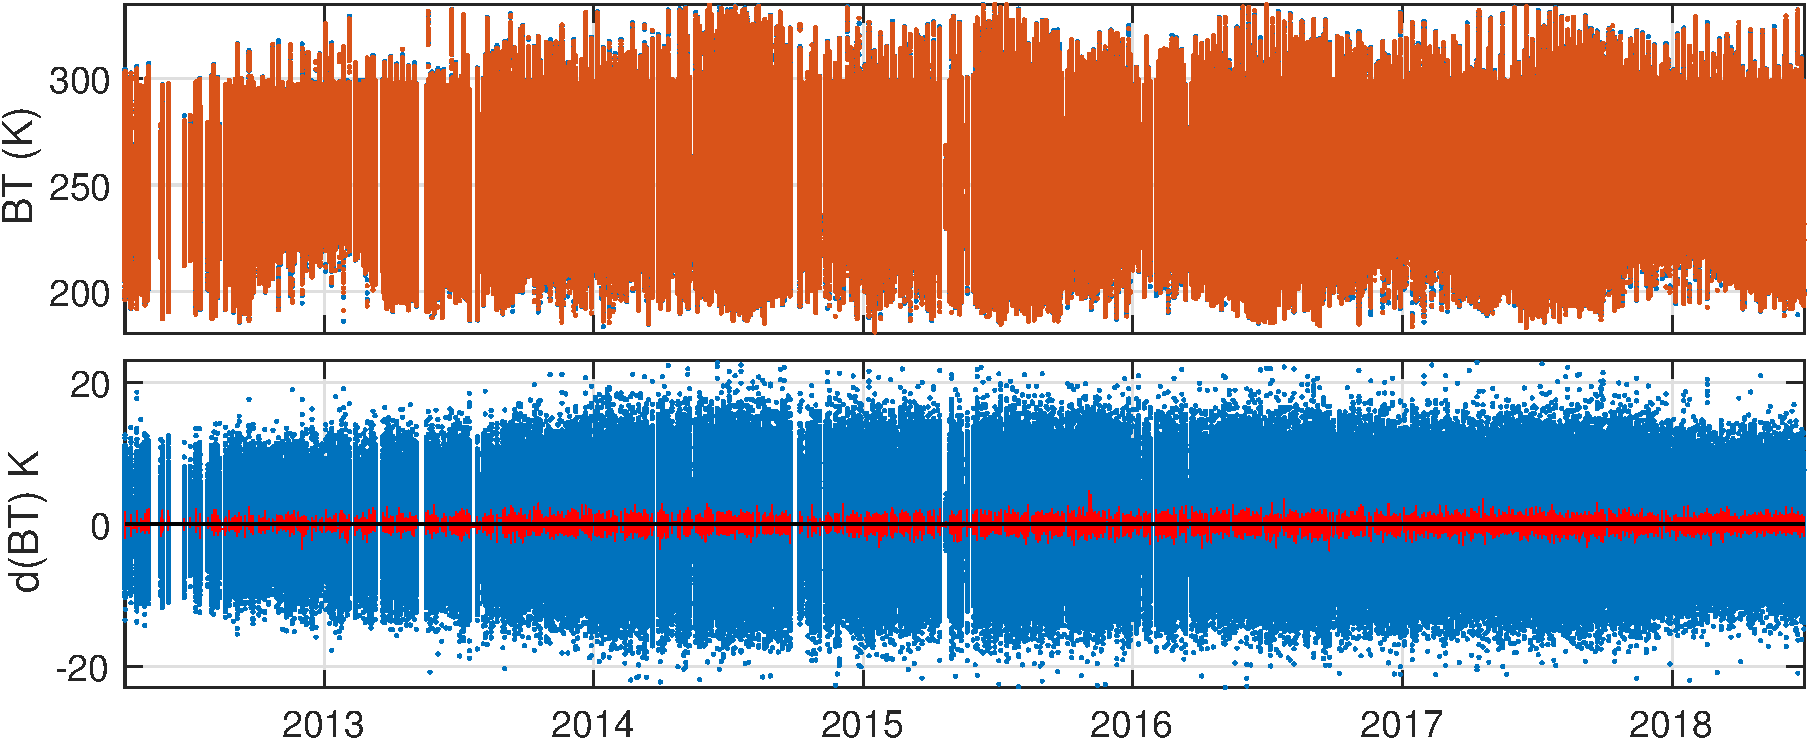
\includegraphics[width=0.66\linewidth]{./Figs/sno_ac1_lr_lw_window_trend_2012_18.png}}
    
%     \subfloat[]{
%       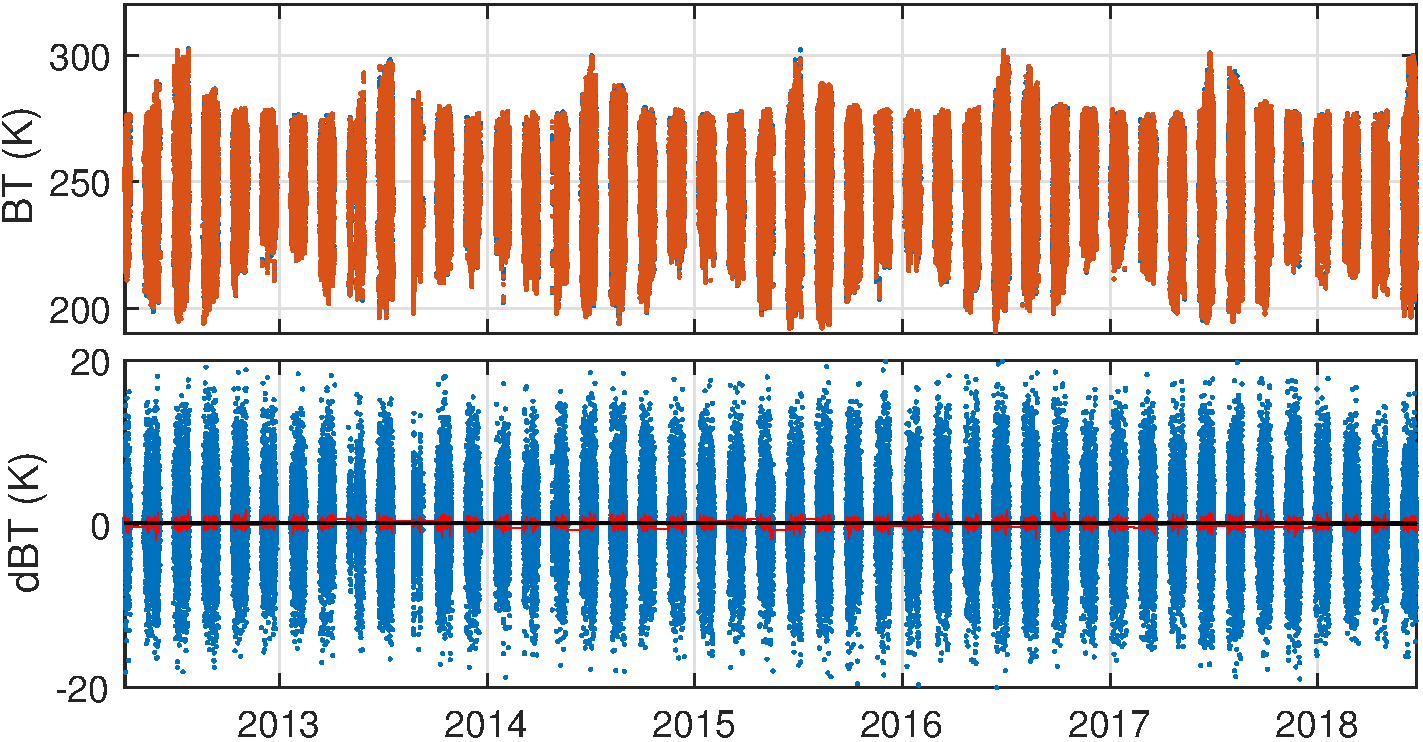
\includegraphics[width=0.66\linewidth]{./Figs/sno_i1c1_lr_lw_window_trend.png}}
%     \end{figure}
    
% \end{frame}

\begin{frame}
  \frametitle{A "CHIRP" Time Series Test}
  \begin{itemize}
  \item Need to connect AIRS to CrIS for long-term hyperspectral sounder time series
  \item We are proposing ``CHIRP'', where AIRS is converted to some form of the CrIS ILS (0.8/0.6/0.4 OPD).
  \item Here we do a simple first test: (using CrIS NSR ILS)
    \begin{itemize}
    \item Create a 10-year time series with AIRS (converted to CrIS ILS: AIRS2CrIS)
    \item Create a 5-year time series with CrIS
    \item Radiometrically adjust (bias) AIRS2CrIS to CrIS using a single static global bias offset (see earlier slides)
    \item Merge 1st 5-years of AIRS2CrIS with the CrIS 5-year time series to create a CHIRP test time series
    \item Intercompare trends from these two time series
    \end{itemize}
  \item Final time series:  AIRS2CrIS is 2007-2012, CrIS is 2012-2017
  \end{itemize}
\end{frame}
%--------------------------------------------------------------------
\begin{frame}
  \frametitle{AIRS/CrIS Hybrid Time Series Trends}
  \centering
  \includegraphics[width=0.8\linewidth]{Figs/trend_airs_vs_airs2cris.pdf}
\end{frame}
% --------------------------------------------------------------------
\begin{frame}
  \frametitle{AIRS/CrIS Hybrid Time Series Trends: Without Adjust}
  \centering \includegraphics[width=0.8\linewidth]{Figs/trend_airs_vs_airs2cris_and_wo_adjust.pdf}
\end{frame}
% --------------------------------------------------------------------
\begin{frame}
  \frametitle{\small AIRS/CrIS Hybrid Time Series Trends: Std/Means over Latitude}
  \centering  \includegraphics[width=0.8\linewidth]{Figs/trend_airs_vs_airs2cris_mean_std_diff_over_lat.pdf}
\end{frame}
% --------------------------------------------------------------------
\begin{frame}
  \frametitle{\small AIRS/CrIS Hybrid Time Series Trends: Add Interannual-Variability}
  \centering   \includegraphics[width=0.8\linewidth]{Figs/trend_airs_vs_airs2cris_mean_std_diff_over_lat_and_interannual_var.pdf}
\end{frame}
% --------------------------------------------------------------------
\begin{frame}
  \frametitle{Latitude Dependent Trends of 902 \wn Window Channel}
  \centering   \includegraphics[width=0.8\linewidth]{Figs/trend_airs_vs_airs2cris_ch902wn_pm80deglat.pdf}

\small Note issue in Arctic.  Maybe too low sampling (due to equal area?).  
\end{frame}

% --------------------------------------------------------------------
\begin{frame}
  \frametitle{Summary}
  \begin{itemize}
  \item Radiometric differences are small between all instruments, but large at the climate level.
  \item We use SNOs and large random (equal area weighted) statistical samples to inter-calibrate (radiometry).
  \item Instruments all appear very stable, so these differences can be account for.
  \item (If) we have enough overlap (true so far) the uncertainty in instrument differences is /very/ small, maybe <0.03K?
  \item Over 5-years that is <0.01K.
  \item Early hybrid (``CHIRP'') time series tests are encouraging.
    
  \end{itemize}
  
\end{frame}
% --------------------------------------------------------------------
%
%trend_airs_vs_airs2cris_ch902wn_pm50deglat.pdf
% trend_airs_vs_airs2cris_std_diff_over_lat.pdf


\end{document}

%%% Local Variables:
%%% mode: latex
%%% TeX-master: t
%%% End:


% --------------------------------------------------------------------
\begin{frame}
  \frametitle{AIRS:CrIS Summary: LW Radiometric}
  \begin{itemize}
  \item Do AIRS SRF functions need adjustment:
    \item First, apply exact $\nu$ calibration to L1c (easy, just didn't do it)
      - ~8 $\wn$ "fringes" in CrIS-AIRS.  Entrance filter fringe shifts?
    \item Try ILS changes that are within estimated TVAC errors
    \item Then, apply as offsets in AIRS2CRIS
    \item \textcolor{maroon}{Testing does NOT require RTA calculations!}  AIRS ILS functions embedded in AIRS2CrIS algorithm.
      
  \end{itemize}
  
\end{frame}
% --------------------------------------------------------------------
\begin{frame}
  \frametitle{AIRS:CrIS SNO showing LW (mod 12) Variability}
  \begin{center}
    \includegraphics[width=0.95\linewidth]{./Figs/sno_ac1_lr_lw_2018d007e040_mean_bias.pdf}
  \end{center}
  
\end{frame}
% --------------------------------------------------------------------
\begin{frame}
  \frametitle{IASI:CrIS SNO showing LW detail}
  \begin{center}
    \includegraphics[width=0.8\linewidth]{./Figs/sno_i1c1_2018q1_lr_lw_mean_bias_null.pdf}
  \end{center}
  
\end{frame}
% --------------------------------------------------------------------
